\documentclass{article}
\usepackage{canvasmathstyle}


\title{Module 3: The Derivative}
\author{Calculus I}
\date{}

\begin{document}

\maketitle

\section{The Definition of the Derivative}

Calculus is fundamentally about the study of change. To understand instantaneous change, we build upon the concept of limits.

% --- DEFINITION CARD ---
\begin{definition}[The Derivative]
    The derivative of a function $f$ at a number $a$, denoted by $f'(a)$, is
    \[
        f'(a) = \lim_{h \to 0} \frac{f(a+h) - f(a)}{h}
    \]
    provided this limit exists.
\end{definition}

% --- OBSERVATION CARD ---
\begin{observation}
    Geometrically, $f'(a)$ represents the \textbf{slope of the tangent line} to the curve $y=f(x)$ at the point $(a, f(a))$.
\end{observation}

% --- TIKZ GRAPHIC ---
% This will become an SVG in your HTML output
\begin{center}
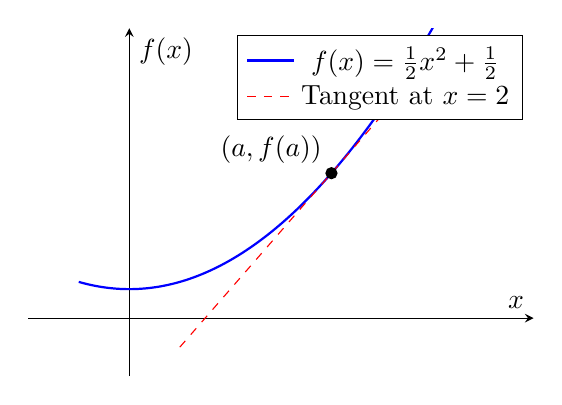
\begin{tikzpicture}
    \begin{axis}[
        axis lines = middle,
        xlabel = $x$,
        ylabel = {$f(x)$},
        ymin=-1, ymax=5,
        xmin=-1, xmax=4,
        width=8cm, height=6cm,
        ticks=none
    ]
        % The Function
        \addplot [blue, thick, domain=-0.5:3.5, samples=100] {0.5*x^2 + 0.5};
        \addlegendentry{$f(x) = \frac{1}{2}x^2 + \frac{1}{2}$}
        
        % The Tangent Line at x=2
        % f(2) = 2.5, f'(2) = 2. Slope = 2.
        % y - 2.5 = 2(x - 2) => y = 2x - 4 + 2.5 => y = 2x - 1.5
        \addplot [red, dashed, domain=0.5:3] {2*x - 1.5};
        \addlegendentry{Tangent at $x=2$}
        
        % The Point
        \addplot[mark=*] coordinates {(2,2.5)};
        \node[above left] at (axis cs:2,2.5) {$(a, f(a))$};
    \end{axis}
\end{tikzpicture}
\end{center}

% --- WARNING CARD ---
\begin{warning}
    \textbf{Differentiation implies Continuity, but not vice versa.}
    Just because a function is continuous at a point does not mean it is differentiable there. 
    Think of the absolute value function $f(x) = |x|$ at $x=0$. It has a sharp corner, so no unique tangent line exists.
\end{warning}

\section{Rules of Differentiation}

Calculating limits every time is tedious. We use theorems to speed up the process.

% --- THEOREM CARD ---
\begin{theorem}[The Power Rule]
    If $n$ is a positive integer, then
    \[
        \frac{d}{dx}(x^n) = nx^{n-1}
    \]
\end{theorem}

% --- PROOF (Standard Environment) ---
\begin{proof}
    We use the Binomial Theorem to expand $(x+h)^n$:
    \begin{align*}
        \frac{d}{dx}(x^n) &= \lim_{h \to 0} \frac{(x+h)^n - x^n}{h} \\
        &= \lim_{h \to 0} \frac{(x^n + nx^{n-1}h + \dots + h^n) - x^n}{h} \\
        &= \lim_{h \to 0} (nx^{n-1} + \text{terms with } h) \\
        &= nx^{n-1}
    \end{align*}
\end{proof}

% --- EXAMPLE CARD ---
\begin{example}
    Find the derivative of $f(x) = x^4 - 2x^2 + 7$.
    
    \textbf{Solution:}
    Using the Power Rule and the Constant Rule:
    \[
        f'(x) = \frac{d}{dx}(x^4) - 2\frac{d}{dx}(x^2) + \frac{d}{dx}(7)
    \]
    \[
        f'(x) = 4x^3 - 2(2x) + 0 = 4x^3 - 4x
    \]
\end{example}

% --- PROCEDURE CARD ---
\begin{algorithm}[Finding Extrema]
    To find local maxima and minima:
    \begin{enumerate}
        \item Find $f'(x)$.
        \item Set $f'(x) = 0$ and solve for $x$ (Critical Points).
        \item Check where $f'(x)$ is undefined.
        \item Use the First Derivative Test to classify the points.
    \end{enumerate}
\end{algorithm}

\begin{aside}[Historical Note]
    \textbf{Newton, Leibniz, and the Notation of Calculus}
    
    Calculus was developed independently in the late 1600s by Isaac Newton and Gottfried Wilhelm Leibniz. Newton approached derivatives through “fluxions,” emphasizing changing quantities over time, while Leibniz introduced the differential notation \(\frac{dy}{dx}\), which remains standard in most calculus texts today. Their competing priority claims led to a long dispute, but modern historians generally emphasize the independent nature of their work and the lasting influence of Leibniz’s notation on teaching and communication in mathematics.\cite{boyer2011history}
\end{aside}

\bibliographystyle{unsrt}
\bibliography{references}

\end{document}